\documentclass[conference,a4paper]{IEEEtran}
\usepackage{amsmath,booktabs,url,cite,graphicx,xcolor}
\usepackage{iftex}
\ifPDFTeX
\usepackage{mathptmx}
\else
\usepackage{fontspec}
\IfFontExistsTF{TeX Gyre Termes}
  {\setmainfont{TeX Gyre Termes}}
  {\setmainfont{Times New Roman}}
\fi
\usepackage[a4paper,left=44.65pt,right=44.65pt,top=27pt,bottom=72pt,columnsep=18pt]{geometry}
\usepackage{balance}
\usepackage{array,tabularx,tikz,pgfplots}
\usetikzlibrary{arrows.meta,positioning,fit}
\pgfplotsset{compat=1.18}
\definecolor{paperBlue}{HTML}{0072B2}
\definecolor{paperTeal}{HTML}{009E73}
\definecolor{paperOrange}{HTML}{D55E00}
\definecolor{paperInk}{HTML}{243746}
\definecolor{paperLight}{HTML}{F2F6FA}
\newcolumntype{Y}{>{\raggedright\arraybackslash}X}
\newcommand{\pct}[1]{#1\%}
\newcommand{\paperAuthor}[3]{%
\begin{minipage}[t]{.318\textwidth}\vspace{0pt}\centering
\parbox[t][25pt][t]{\linewidth}{\centering\fontsize{10}{11}\selectfont #1}\par
{\fontsize{8.5}{10}\selectfont\itshape #2\\
Department of Computer Science and Engineering\\
Koneru Lakshmaiah Education Foundation\\
Bowrampet, Hyderabad-500043, Telangana, India\par}
\vspace{2pt}{\fontsize{8}{9}\selectfont\texttt{#3}\par}
\end{minipage}}
\title{AI-Driven Adaptive Quantum-Resilient Security Framework for Secure Microservice Architectures}
\author{\begin{minipage}{\textwidth}\centering
\paperAuthor{Yellanki Kranthi Giri Venkata Chary}{Student}{y.kranthi826@gmail.com}\hfill
\paperAuthor{Morampudi Girish Venkat Sai}{Student}{girishrocks1818@gmail.com}\hfill
\paperAuthor{Velthuru Vinisha}{Project Guide}{vinisha.velthuru0216@gmail.com}
\par\vspace{12pt}
\paperAuthor{Alla Sai Harsha}{Student}{allasaiharsha15@gmail.com}\hspace{.06\textwidth}
\paperAuthor{ Billa Venkateshewara Laxmana}{Student}{l45115984@gmail.com}
\end{minipage}}
\begin{document}
\maketitle
\begin{abstract}
Microservice security requires distinct controls for identity, threat observation, cryptographic protection, and operational accountability. This paper presents a research prototype connecting these functions through a versioned adaptive policy. A Java service architecture combines gateway authentication, network-flow inference, profile selection, signed encrypted envelopes, and MySQL execution records. Classical, hybrid, and post-quantum profiles share an interface; incompatible high-risk requests fail rather than silently receive classical protection. Evaluation separates classification from functional security checks. The retained Random Forest reaches 89.79\% accuracy on the official UNSW-NB15 test partition, with 19.85\% false positives. A bounded CICIoT2023 study rejects both evaluated binary models, and grouped microservice syscall studies produce no eligible replacement. Controlled routed HTTP experiments show a matched-pipeline improvement but miss their recall release gate. Actual-service checks verify round trips, identity-linked records, and downgrade denials. Controlled persistence failures demonstrate that verified cryptography and successful request completion require separate reporting. These findings support a reproducible integration prototype while exposing detection and deployment limitations; they do not establish universal attack prevention or end-to-end quantum-resilient transport.
\end{abstract}
\begin{IEEEkeywords}
microservice security, post-quantum cryptography, intrusion detection, crypto agility, audit persistence
\end{IEEEkeywords}
\section{Introduction}
An intrusion score estimates suspiciousness; authorization determines permitted access; cryptographic verification checks a message. These are complementary controls, not interchangeable evidence of security. NIST microservice guidance addresses identity, discovery, key management, communication, throttling, and monitoring~\cite{mesh}. The cryptographic profiles draw on ML-KEM and ML-DSA specifications~\cite{kem,dsa}. Our application-level integration does not implement a complete service mesh.

\subsection{Problem and Motivation}
Microservices divide an application into independently managed capabilities, but a request can still cross several trust boundaries before its business operation completes~\cite{mesh}. Gateway and transport configuration also change the performance boundary around those controls~\cite{gateway}. A valid login at an ingress point does not make later dependencies trustworthy. Conversely, an unusual traffic pattern is not sufficient evidence that an authenticated user should be denied access. An adaptive security framework must connect observations to actions without erasing these distinctions. Otherwise, an attractive dashboard can report protection even when the underlying request failed or the selected mechanism did not address the observed threat.

Quantum migration adds a different planning problem. Long-lived information may require protection against future decryption of material collected today~\cite{readiness,enterprise}. That requirement is not determined solely by the probability that the current request is malicious. A low-scored request can carry highly sensitive information, while an obvious flooding request may carry no confidential payload at all. Detection and cryptographic migration therefore operate on related but different dimensions. This study keeps sensitivity and compatibility visible rather than treating an intrusion score as a complete security policy.

The practical difficulty is not merely choosing between three algorithm names. The selected profile must correspond to an executable implementation, its decision must be checked at the execution boundary, and its outcome must remain distinguishable from the outcomes of persistence and monitoring. A service can produce and verify an envelope, then fail to commit its completion record. Treating that operation as either a wholly successful protection or as proof that cryptography never ran would mislead an operator. We examine this intermediate state explicitly.

\subsection{Research Questions and Contributions}
The investigation is organized around four questions. RQ1 asks whether a versioned policy can select implemented classical, hybrid and PQC profiles while refusing a tested unsafe downgrade. RQ2 asks how detection performance changes across official network partitions, bounded IoT traffic, grouped microservice observations and routed HTTP contexts. RQ3 asks which outcomes remain knowable when cryptography, persistence and monitoring do not succeed together. RQ4 asks what a matched local envelope benchmark can establish without implying a production speedup.

The first contribution is an executable integration of service-owned identity, policy, inference, cryptographic execution and audit records. The second is an evidence-oriented evaluation in which final tests, development ablations and functional checks remain separate. The third is a failure model that preserves verified cryptography without labeling a failed request successful. The fourth is a measured characterization of complete local envelopes, including key generation, verification and component sizes. These are integration and empirical contributions. We neither introduce a cryptographic primitive nor establish a state-of-the-art detector.

\subsection{Scope of the Claim}
The application is a local research security platform with a web dashboard, not a replacement operating system, universal firewall or externally validated security appliance. Its Business Service is the demonstration integration target. Other applications would require adapters, authenticated telemetry, appropriate identity and key management, and a workload-specific evaluation. The word adaptive refers to constrained profile selection; it does not mean that every suspicious request is blocked or that the model learns online from unreviewed traffic.

The remainder of this paper first positions the work within the retained literature. It then describes the architecture, policy and evidence model, followed by dataset-specific protocols. Results include unsuccessful candidates because release decisions are part of the research outcome. The discussion separates established behavior from operational requirements that remain untested. Reproduction details and interpretation rules are provided in the appendices rather than relying on project screenshots as evidence.

\section{Related Work}
UNSW-NB15 supplies network features and predefined partitions~\cite{unsw}. CICIoT2023 supplies a different IoT environment including flooding, reconnaissance, brute-force and web attack categories~\cite{ciciot}. Neither dataset alone validates application-specific microservice detection.

Flora and Antunes provide a microservice benchmark and public dataset~\cite{flora,dataset}. Their evaluation compares six detectors across application and deployment scenarios, including version changes. Our bounded SocialNetwork study preserves recording and vulnerability-group boundaries; exposure annotations do not certify malicious behavior in every window. It does not reproduce their complete benchmark or establish a superior detector.

Stasac et al. evaluate risk-based encryption selection for web applications~\cite{adaptive}. Their proposed weight configuration correctly assigns all 27 designed scenarios to expected risk zones. Their separate CSIC2010 held-out evaluation has 21,065 requests: Table 26 reports 65.1\% zone accuracy and 77.7\% attack recall at the selected operating point. These results concern different experiments. The scenario result is neither an operational intrusion-detection accuracy nor a directly matched baseline for this project. Our current contribution concerns auditable execution across classical, hybrid and PQC profiles; a matched adaptive-versus-static system comparison remains open.

Binh et al. combine SAGEConv graph learning and a Transformer~\cite{sage}. Their UNSW-NB15 mean accuracy is 98.41\% with a standard deviation of 0.06 percentage points over five seeds. They use approximately 100,000 sampled flows, time-based splits, graph construction and contextual features. Our official predefined-partition RF result is numerically lower, but protocol differences prevent a controlled ranking or an improvement claim. Adopting their architecture would require compatible graph observations and a new frozen evaluation.

Olushola and Meenakshi investigate authenticated sessions using ML-KEM-1024, ML-DSA-65 and AES-256-GCM~\cite{session}. Their protocol binds endpoint authentication and key derivation to session transcripts. Our local ML-KEM-768 or hybrid envelope checks do not reproduce that endpoint-authenticated session boundary. Primitive and handshake timings from their Python/C environment cannot be ranked against our Java API timings without matching operation scope, payload, key lifecycle and hardware.

Matias et al. evaluate gateway/JWT and HTTPS configurations in a three-service testbed, reporting response-time distributions across 54 benchmark cases~\cite{gateway}. This motivates measuring security overhead, but is not a source of detection accuracy. We do not adopt removal of internal transport protection as an optimization. Our current bounded local service checks likewise do not prove secure production transport.

\subsection{Lifecycle, Migration and Explainability}
The retained NIST DevSecOps publication is SP 800-204C, issued in March 2022~\cite{devsecops}. It distinguishes application code, application-services code, infrastructure as code, policy as code and observability as code. This distinction is useful here: validating a classifier does not validate deployment configuration, and compiling a service does not validate its monitoring rules. Our versioned protocols and regression evidence follow that lifecycle separation. The prototype is not a Kubernetes service-mesh implementation or a demonstration of continuous authority to operate.

Inakollu discusses quantum-resilient enterprise and cloud architectures, including algorithm abstraction, migration planning and hybrid operation~\cite{enterprise}. We use this source as architectural context, not as empirical evidence that the present system prevents quantum attacks. Its enterprise-analysis claims have not been independently reproduced in this study. In particular, a predicted date for cryptographically relevant quantum computing is not needed to interpret our local envelope experiments. The relevant engineering concern is whether a system can identify and replace cryptographic dependencies while retaining compatibility and accountability.

Gupta and Mittal separate retroactive confidentiality loss from future authentication and integrity risks in enterprise-cloud transition planning~\cite{readiness}. Their quantitative exposure estimates depend on confidentiality lifetime, migration duration and an assumed distribution of quantum-computer availability. These are planning-model outputs, not intrusion-detection accuracy. Their treatment motivates a long-term requirement that is absent from a traffic-only policy: information that remains sensitive for years should not receive weaker confidentiality simply because its current request looks normal. Our present sensitivity field is only a prototype input; a production design must obtain it from an authoritative resource policy.

Asghari Varzaneh and Hosseini propose binary Levy-opposition-equilibrium optimization for network feature selection~\cite{feature}. Their KNN-based evaluation uses random ten-fold partitions and repeated optimization runs. It reports 97.6\% UNSW-NB15 accuracy with an average 10.8 selected features. The feature count is an average, not an implementable fractional vector. This study supports investigating informative representations, but does not provide a matched comparison with our official predefined test. Repeating feature selection after viewing the official test would compromise that comparison rather than strengthen it.

Sharma et al. combine self-attention, learnable feature gating and SHAP/LIME explanations~\cite{xai}. They report 99.3\% on BoT-IoT, 99.6\% on N-BaIoT and 97.9\% on UNSW-NB15. Their stated random 70/15/15 partitions and multi-category setting differ from the predefined binary protocol used here. We treat those figures as author-reported results, not scores reproduced by this project. A transparent policy explanation and a feature-attribution explanation also answer different questions. Our dashboard can describe the selected mode and recorded risk; this does not amount to implementing or validating their explanation framework.

\subsection{Research Gap and Comparison Discipline}
Table~\ref{literature} maps all eleven retained sources to the present study. The gap is deliberately narrower than claiming that adaptive security, microservice IDS or PQC integration is new. The reviewed sources emphasize different units of evaluation: risk zones, classified flows, syscall traces, authenticated sessions, gateway latency, lifecycle controls or migration exposure. A practical integration must preserve those units while showing what actually happened to one business operation. This paper studies that join and its failure semantics.

\begin{table*}[t]
\caption{Scope-matched use of the eleven retained sources. Reported percentages are not matched baselines for this prototype.}
\label{literature}\centering\footnotesize
\begin{tabularx}{\textwidth}{|p{.13\textwidth}|p{.24\textwidth}|Y|Y|}\hline
Source & Main unit of evaluation & Relevance to this study & Boundary of comparison\\\hline
Stasac et al.~\cite{adaptive}, 2026 & Designed risk zones; separate CSIC requests & Risk-dependent algorithm selection & 100\% on 27 designed scenarios is not operational IDS accuracy\\\hline
Binh et al.~\cite{sage}, 2026 & Sampled time-split graph flows & Relational detection context & 98.41\% mean uses a different representation and split\\\hline
Flora and Antunes~\cite{flora}, 2024 & Microservice traces and deployment scenarios & Public syscall observations and grouped evaluation & Present subset does not reproduce the complete benchmark\\\hline
Olushola and Meenakshi~\cite{session}, 2026 & Authenticated PQC session & Transcript and endpoint identity requirements & Local envelope round trips are not that session protocol\\\hline
NIST SP 800-204C~\cite{devsecops}, 2022 & Lifecycle and service-mesh guidance & Policy and observability under version control & Guidance, not a detector percentage or a conformance certificate\\\hline
Matias et al.~\cite{gateway}, 2024 & Gateway/JWT/HTTPS workload cases & Performance boundaries around authentication & Request latency is not classification accuracy\\\hline
NIST FIPS 203~\cite{kem}, 2024 & Key encapsulation specification & Standardized ML-KEM parameter sets & Algorithm specification does not certify this application\\\hline
Inakollu~\cite{enterprise}, 2025 & Enterprise architecture and migration & Crypto-agility and deployment context & Architectural claims are not independently reproduced here\\\hline
Asghari Varzaneh and Hosseini~\cite{feature}, 2024 & KNN feature-subset search & Representation and optimization choices & Random ten-fold results are not the official test protocol\\\hline
Sharma et al.~\cite{xai}, 2025 & Attention-based classification/explanation & Detection interpretability & Different datasets, labels and random partitions\\\hline
Gupta and Mittal~\cite{readiness}, 2026 & Migration exposure simulation & Confidentiality lifetime and uncertainty & Exposure fraction is not an observed attack detection rate\\\hline
\end{tabularx}
\end{table*}

Our approach complements rather than replaces these lines of work. Network classifiers inform one observation channel; syscall studies reveal whether another channel observes the relevant behavior; cryptographic profiles protect an envelope; and lifecycle controls govern deployment. The unresolved issue is how to combine these capabilities without presenting one successful component as evidence that the entire chain is secure. We address a tested part of that issue through explicit contracts, consistent identifiers, rejection gates and records of negative experiments.

The retained library is a project-focused selection, not a systematic review with a preregistered search strategy. We therefore do not infer the absence of similar systems from this collection. A publication claiming algorithmic novelty would need a broader search and matched reproduction. The defensible research position here is a transparent systems study with reusable evaluation boundaries and documented integration limitations.

\section{Methodology}
\subsection{System Design}
API Gateway, Auth, Business, Security Monitoring, Adaptive Policy, AI Security and Eureka discovery comprise the local system. Spring supports Java services, Python serves inference, MySQL stores service-owned records, and React displays API snapshots and restricted operator alerts.

Figure~\ref{architecture} distinguishes the request path from the observation path. Gateway exposes application routes; Auth registers and authenticates users; Business executes the protected demonstration operation. Policy requests a score from AI Security and persists its decision. Monitoring receives security events through internal interfaces and makes authorized snapshots available. Discovery locates services; it does not establish their authorization. Internal API credentials are separate from user bearer tokens, and administrative monitoring access is separate from ordinary business access.

\begin{figure*}[t]
\centering
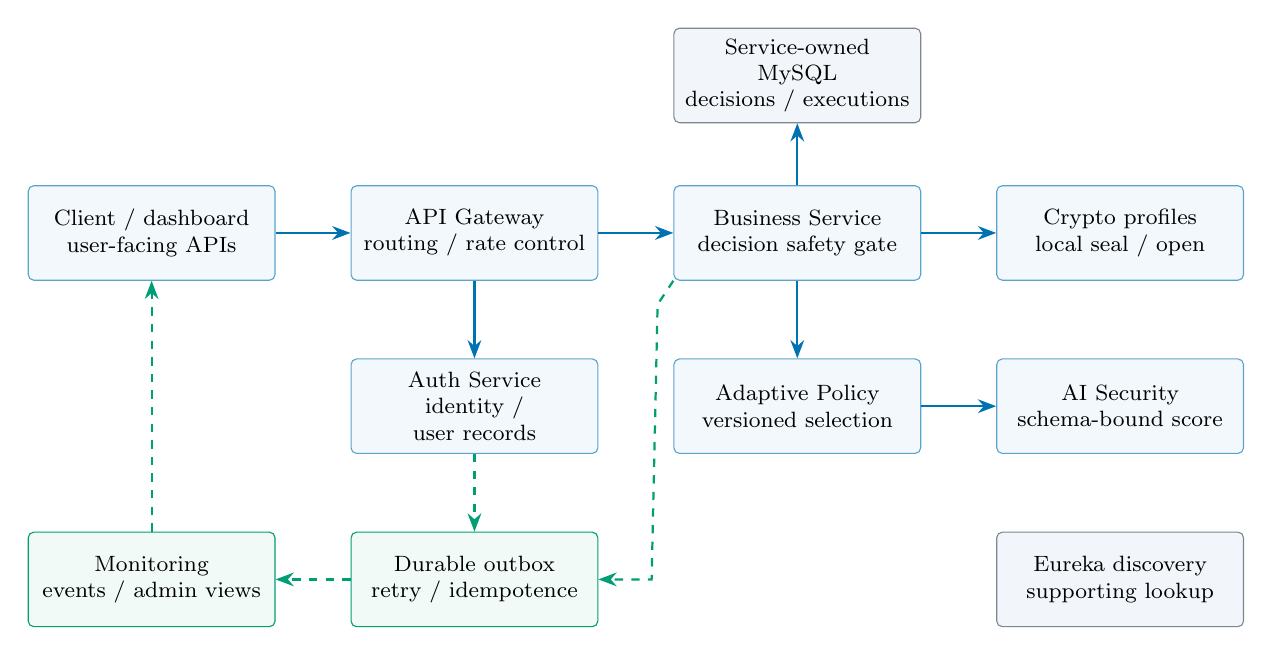
\begin{tikzpicture}[>=Stealth,
 box/.style={draw=paperBlue!65,fill=paperBlue!5,rounded corners=2pt,align=center,font=\footnotesize,minimum height=12mm,text width=29mm},
 call/.style={->,thick,draw=paperBlue},
 audit/.style={->,thick,dashed,draw=paperTeal}]
\node[box] (client) at (0,0) {Client / dashboard\\user-facing APIs};
\node[box] (gateway) at (4.1,0) {API Gateway\\routing / rate control};
\node[box] (business) at (8.2,0) {Business Service\\decision safety gate};
\node[box] (crypto) at (12.3,0) {Crypto profiles\\local seal / open};
\node[box] (auth) at (4.1,-2.2) {Auth Service\\identity / user records};
\node[box] (policy) at (8.2,-2.2) {Adaptive Policy\\versioned selection};
\node[box] (ai) at (12.3,-2.2) {AI Security\\schema-bound score};
\node[box,draw=paperInk!60,fill=paperLight] (db) at (8.2,2.0) {Service-owned MySQL\\decisions / executions};
\node[box,draw=paperTeal,fill=paperTeal!5] (monitor) at (0,-4.4) {Monitoring\\events / admin views};
\node[box,draw=paperTeal,fill=paperTeal!5] (outbox) at (4.1,-4.4) {Durable outbox\\retry / idempotence};
\node[box,draw=paperInk!60,fill=paperLight] (discovery) at (12.3,-4.4) {Eureka discovery\\supporting lookup};
\draw[call] (client)--(gateway);
\draw[call] (gateway)--(business);
\draw[call] (gateway)--(auth);
\draw[call] (business)--(crypto);
\draw[call] (business)--(policy);
\draw[call] (policy)--(ai);
\draw[call] (business)--(db);
\draw[audit] (auth)--(outbox);
\draw[audit] (business.south west)-- ++(-2mm,-3mm) -- (6.35,-4.4) -- (outbox.east);
\draw[audit] (outbox)--(monitor);
\draw[audit] (monitor)--(client);
\end{tikzpicture}
\caption{Implemented architecture. Blue solid arrows denote logical requests or writes; teal dashed arrows denote audit publication and retrieval. The database box summarizes service-owned storage, not a shared cross-service transaction. Discovery supports lookup and does not establish trust. Arrows summarize responsibilities rather than every network call.}
\label{architecture}
\end{figure*}

\subsubsection{Threat model}
The evaluated adversarial actions include missing or invalid bearer credentials, bounded repeated authentication attempts and incompatible high-risk profile requests. The classification studies additionally cover labeled network attacks, controlled suspicious HTTP intent and annotated syscall exposure. These sources do not describe an identical attacker. A valid application request may coexist with a high network score, and an invalid token can arise from an ordinary user mistake. Decisions must retain the distinction between authentication evidence and model evidence.

For cryptographic testing, the implementation checks envelope integrity and recovered plaintext under locally generated keys. A remote active attacker, compromised provider, stolen signing key, malicious dependency or compromised host is outside the demonstrated round-trip guarantee. Database outages and controlled transaction failures are operational fault cases, not automatically attributed to an attacker. The alerting experiment uses a synthetic counter signal and cannot establish the cause of a real incident.

\subsubsection{Assets and trust boundaries}
The relevant assets are credentials, payload confidentiality, envelope integrity, execution records and the reliability of operator information. User-facing endpoints and internal service interfaces form separate boundaries. MySQL service ownership limits responsibility: a monitoring event is not a substitute for a Business execution record, and a stored policy decision is not proof that Business executed it. Identifiers connect these records for verification; they do not create an atomic transaction across all services.

Secrets are supplied through local configuration rather than embedded in evidence reports. Dataset and model artifacts are kept separately from tracked source. The study receipts avoid plaintext payloads, private keys and bearer credentials. A payload fingerprint supports equality checks across receipts, but hashing is not anonymization for predictable low-entropy content. The demonstration uses synthetic payloads to avoid making a confidentiality claim about real customer information.

The adaptive endpoint accepts payload, flow features, sensitivity, capabilities and a latency hint. Policy combines model score with application constraints. Business validates decision identity, score, effective risk, compatibility and exact profile before execution. Caller-supplied features and sensitivity are not trusted sensor observations; server-owned constraints remain future acceptance work. Figure~\ref{workflow} follows one operation through these boundaries, separating unsafe-decision refusal from verified cryptographic execution.

\begin{figure*}[t]
\centering
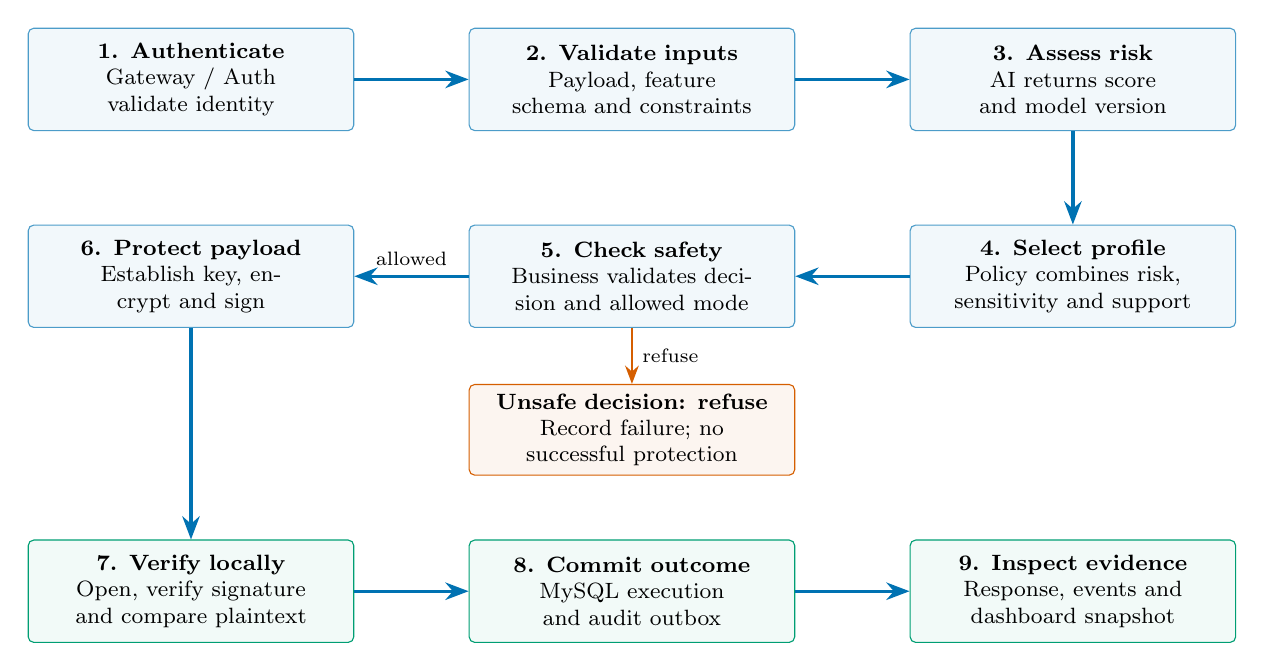
\begin{tikzpicture}[>=Stealth,
 wfstep/.style={draw=paperBlue!70,fill=paperBlue!5,rounded corners=2pt,text width=39mm,minimum height=13mm,align=center,font=\footnotesize},
 flow/.style={->,very thick,draw=paperBlue},
 reject/.style={draw=paperOrange,fill=paperOrange!6,rounded corners=2pt,text width=39mm,minimum height=10mm,align=center,font=\footnotesize}]
\node[wfstep] (s1) at (0,0) {\textbf{1. Authenticate}\\Gateway / Auth validate identity};
\node[wfstep] (s2) at (5.6,0) {\textbf{2. Validate inputs}\\Payload, feature schema and constraints};
\node[wfstep] (s3) at (11.2,0) {\textbf{3. Assess risk}\\AI returns score and model version};
\node[wfstep] (s4) at (11.2,-2.5) {\textbf{4. Select profile}\\Policy combines risk, sensitivity and support};
\node[wfstep] (s5) at (5.6,-2.5) {\textbf{5. Check safety}\\Business validates decision and allowed mode};
\node[wfstep] (s6) at (0,-2.5) {\textbf{6. Protect payload}\\Establish key, encrypt and sign};
\node[reject] (deny) at (5.6,-4.45) {\textbf{Unsafe decision: refuse}\\Record failure; no successful protection};
\node[wfstep,draw=paperTeal,fill=paperTeal!5] (s7) at (0,-6.5) {\textbf{7. Verify locally}\\Open, verify signature and compare plaintext};
\node[wfstep,draw=paperTeal,fill=paperTeal!5] (s8) at (5.6,-6.5) {\textbf{8. Commit outcome}\\MySQL execution and audit outbox};
\node[wfstep,draw=paperTeal,fill=paperTeal!5] (s9) at (11.2,-6.5) {\textbf{9. Inspect evidence}\\Response, events and dashboard snapshot};
\draw[flow] (s1)--(s2);
\draw[flow] (s2)--(s3);
\draw[flow] (s3)--(s4);
\draw[flow] (s4)--(s5);
\draw[flow] (s5)--node[above,font=\scriptsize]{allowed}(s6);
\draw[flow] (s6)--(s7);
\draw[flow] (s7)--(s8);
\draw[flow] (s8)--(s9);
\draw[->,thick,draw=paperOrange] (s5)--node[right,font=\scriptsize]{refuse}(deny);
\end{tikzpicture}
\caption{End-to-end adaptive workflow. Numbered stages show control order; the orange branch is a refusal, not a successful classical fallback. Initial persistence precedes policy/cryptography in the implementation. A failed completion write follows the fault paths in Fig.~\ref{auditstate}, so stage 7 alone does not establish stage 8 or a successful response.}
\label{workflow}
\end{figure*}

\subsection{Constrained Decision and Execution Contract}
Let $x$ denote a schema-valid observation and $s=f_v(x)$ the score produced by model version $v$. Let $r$ denote its discrete risk category, $d$ the supplied sensitivity, $h$ and $q$ the hybrid/PQC capability flags, and $b$ the latency-selection hint. The policy is a versioned mapping
\begin{equation}
 P_w(r,d,h,q,b)=(r_e,m,a,e),
\end{equation}
where $r_e$ is effective risk, $m$ the selected mode, $a$ its exact algorithm profile and $e$ the recorded reason. This notation describes the implementation contract; it is not a learned optimization objective. In particular, $s$ is not the probability that cryptographic failure will occur, and $b$ is not a measured runtime bound.

Policy version 1.1.0 elevates a CONFIDENTIAL request by one risk level and forces RESTRICTED data to HIGH. PUBLIC and INTERNAL leave the model category unchanged. HIGH selects PQC when supported with $b\geq15$ ms, otherwise hybrid when supported with $b\geq8$ ms. MEDIUM selects hybrid when supported with $b\geq8$ ms. Remaining branches select classical, including a recorded HIGH fallback when neither stronger option qualifies. Business independently rejects that HIGH/classical combination before cryptographic execution. Recording a selection and authorizing its execution are therefore distinct actions.

The constants 8 and 15 ms are heuristic policy thresholds, not values learned from the JMH measurements reported later. A production optimizer would need workload costs, authenticated capabilities and explicit safety constraints before choosing an objective such as latency or migration coverage. We do not retrospectively fit these constants to the reported benchmark or claim optimality. The tested refusal is more important than silently satisfying a small budget with an unacceptable mode.

Table~\ref{policybranches} presents the executable branch logic without treating all possible caller inputs as trustworthy. Checking a supplied capability flag establishes contract consistency, not endpoint possession of a key. Similarly, accepting a numeric feature vector establishes shape and range requirements, not that the vector was measured from the current request. These limitations constrain the system-level security interpretation even when the branch implementation is correct.

\begin{table}[t]
\caption{Policy branches and separate Business safety gate}
\label{policybranches}\centering\footnotesize
\begin{tabularx}{\columnwidth}{|Y|Y|}\hline
Effective risk and supplied constraints & Selection / execution\\\hline
HIGH; PQC supported; $b\geq15$ ms & PQC; executable\\\hline
HIGH; preceding branch unavailable; hybrid supported; $b\geq8$ ms & Hybrid; executable\\\hline
HIGH; neither branch available & Classical recorded; execution refused\\\hline
MEDIUM; hybrid supported; $b\geq8$ ms & Hybrid; executable\\\hline
LOW, or remaining MEDIUM branch & Classical; executable\\\hline
\end{tabularx}
\end{table}

The Business boundary checks the returned decision before use rather than dispatching any arbitrary algorithm string. It retains model and policy versions, effective risk, execution identity and correlation identity. Unknown or inconsistent profiles fail rather than becoming a default implementation. This limits accidental negotiation drift within the tested application. It does not solve malicious policy compromise or make a caller-controlled sensitivity label authoritative.

\subsection{Cryptographic Execution}
Table~\ref{profiles} lists implemented profiles. AES-256-GCM protects payloads; the PQC building blocks are ML-KEM and ML-DSA~\cite{kem,dsa}. Hybrid key establishment uses the maintained provider's X-Wing composition rather than a custom combiner. Standards citations identify the primitives, not certification of the present application.
\begin{table}[t]
\caption{Implemented cryptographic profiles}\label{profiles}\centering\footnotesize
\begin{tabular}{|l|l|l|}\hline
Mode&Key establishment&Signature\\\hline
Classical&X25519&ECDSA P-256\\\hline
Hybrid&X-Wing&ML-DSA-65\\\hline
PQC&ML-KEM-768&ML-DSA-65\\\hline
\end{tabular}
\end{table}

Each operation generates ephemeral recipient/signing keys, seals and opens the payload, and verifies equality. Associated data binds execution, correlation and policy decision identities. This proves a local round trip, not external-recipient identity, production key delivery or FIPS 140 validation. HIGH-risk classical execution is refused. The latency hint is not a completion deadline. PQC selection does not itself stop flooding.

\subsubsection{Envelope semantics}
The common interface separates key establishment, payload encryption and signing. The Java 21 implementation uses Bouncy Castle 1.86. AES-GCM uses a 96-bit nonce and 128-bit authentication tag; derived payload keys use HKDF-SHA256 in the envelope path. Associated data incorporates execution, correlation and decision context so that integrity is evaluated with the intended operation identifiers. Verification and plaintext-equality checks occur inside the local operation, not through a separate remote recipient.

The shared interface enables a matched operation boundary, but the profiles are not interchangeable security levels on a single numerical scale. The classical profile retains quantum-vulnerable public-key mechanisms. Hybrid uses the provider's maintained X-Wing construction, not a project-designed concatenation rule. The PQC profile uses ML-KEM-768 and ML-DSA-65, while the session work in~\cite{session} uses a different KEM parameter set and an endpoint-authenticated protocol. Provider availability and algorithm names alone do not certify side-channel resistance, lifecycle management or implementation conformance.

Ephemeral signing keys generated and trusted within the same operation cannot identify an independently authenticated sender. Likewise, opening an envelope with a locally generated recipient key does not demonstrate safe distribution of that key to an application elsewhere. The experiment exercises actual cryptographic computation and tamper-sensitive operations, but transport TLS, certificate lifecycle, long-term key storage and recipient authorization require separate integration. This boundary prevents a functional demonstration from being mislabeled end-to-end quantum-safe communication.

\subsection{Persistence and Failure}
Execution audits retain a payload fingerprint, identifiers, versions, mode, timing and outcome, not plaintext or private keys. A durable outbox supports monitoring delivery and explicit recovery.

Initial audit persistence precedes policy and crypto. A failed initial write triggers one sanitized failure-record attempt without policy execution. If crypto succeeds but completion persistence fails, a recovered FAILED record may correctly retain verified=true. If fallback also fails, STARTED does not establish whether crypto ran. The original exception and an in-memory counter preserve limited diagnostics. The dashboard excludes failed requests from successful protection shares. Counter alerts are not durable incident storage: restart or crash before scraping can remove observations.

\subsubsection{State and transaction boundaries}
Figure~\ref{auditstate} summarizes the distinction between an attempted operation and a durably completed one. STARTED means that initiation was recorded. It is not a negative cryptographic result. SUCCESS requires the corresponding successful completion path, while FAILED can preserve verification evidence if the failure occurred later. A transactional completion write and its outbox enqueue can roll back together; a separate fallback then attempts to save the sanitized failure. If both attempts fail, no successful audit is invented.

\begin{figure}[t]
\centering
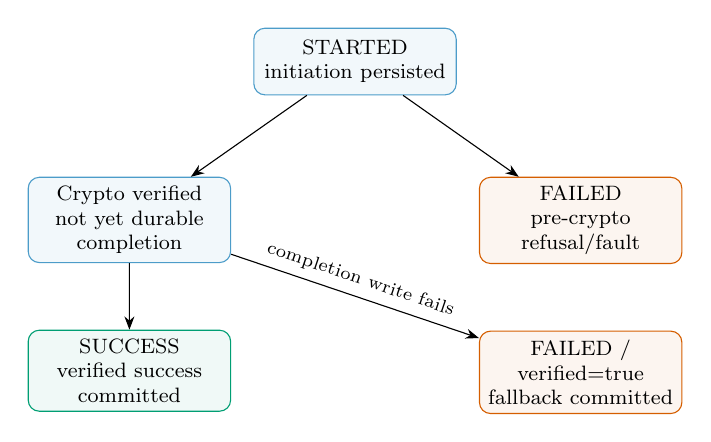
\begin{tikzpicture}[>=Stealth, node distance=9mm,scale=.94,transform shape,
 s/.style={draw=paperBlue!70,fill=paperBlue!5,rounded corners,align=center,font=\footnotesize,text width=25mm,minimum height=9mm}]
\node[s] (start) {STARTED\\initiation persisted};
\node[s,below left=11mm and 3mm of start] (crypto) {Crypto verified\\not yet durable completion};
\node[s,draw=paperOrange,fill=paperOrange!6,below right=11mm and 3mm of start] (fail) {FAILED\\pre-crypto refusal/fault};
\node[s,draw=paperTeal,fill=paperTeal!6,below=of crypto] (complete) {SUCCESS\\verified success committed};
\node[s,draw=paperOrange,fill=paperOrange!6,below=of fail] (late) {FAILED / verified=true\\fallback committed};
\draw[->] (start)--(crypto);
\draw[->] (start)--(fail);
\draw[->] (crypto)--(complete);
\draw[->] (crypto)--node[above,sloped,font=\scriptsize]{completion write fails}(late);
\end{tikzpicture}
\caption{Logical audit states. The intermediate crypto state is not necessarily durable. If completion and fallback both fail, the stored STARTED row remains ambiguous; the diagram does not imply guaranteed terminal-state persistence.}
\label{auditstate}
\end{figure}

A durable outbox decouples a service transaction from later monitoring delivery. Retry and idempotence checks address repeated delivery, not exactly-once execution of every distributed operation. There is no cross-service database transaction joining Auth, Policy, Business and Monitoring. Independent post-run joins instead verify that the recorded identities and versions agree. This is useful evidence of the tested run, while partial failures and crash recovery still require explicit treatment.

The schema separates policy decisions, business executions and security events rather than placing all outcomes in a single log string. Execution records contain a payload fingerprint, selected mode, exact profile, verification flag, timing fields and outcome. Event records describe their source service and request context. Raw payloads and private keys are not part of these research receipts. Operational retention, least-privilege database users, encryption at rest and backup recovery are separate deployment requirements; the existence of a relational schema does not establish them.

\subsubsection{Operator-facing evidence}
The dashboard displays API snapshots with distinct wording for verified success, failed flow and unavailable information. A FAILED record with verification=true is not included in successful-protection shares or successful-flow averages. A missing timing is described as unrecorded rather than as proof that the operation never executed. These choices are part of the information model: presenting incomplete evidence as an absolute claim would obscure the very failure cases the system records.

Operational alerts are restricted to administrator access. A positive in-memory audit-failure counter triggers the tested pending/firing behavior; an unavailable or malformed metric is treated separately from a healthy zero. Unknown monitoring state remains unknown rather than rendering a reassuring empty list. External email delivery and durable incident lifecycle are not established by the local propagation probe. Component tests also do not replace an independent accessibility or browser interaction review.

\subsection{Evaluation Protocols}
Each observation setting has its own preparation and independence protocol, detailed below. We report the target label and support counts with each result rather than pooling incompatible observations.

For binary classification,
\begin{equation}
\mathrm{Accuracy}=\frac{TP+TN}{TP+TN+FP+FN},
\end{equation}
\begin{equation}
\mathrm{Recall}=\frac{TP}{TP+FN},\quad
\mathrm{FPR}=\frac{FP}{FP+TN}.
\end{equation}
Macro-F1 averages class-specific F1. Frozen recipes, hashes, confusion matrices and rejected candidates are retained. Functional checks are not classifier accuracy.

\subsection{Dataset Provenance and Feature Management}
Table~\ref{datasets} summarizes the four observation settings, with public provenance supplied by the original UNSW-NB15, CICIoT2023 and microservice releases~\cite{unsw,ciciot,flora,dataset}. The datasets are not concatenated into one training matrix. An UNSW flow, a CIC traffic statistic, a SocialNetwork syscall window and a gateway request history do not represent the same measurement. Giving them similar column names would not create semantic compatibility. The deployed historical network model remains separate from experimental detectors built for other schemas.

\begin{table*}[t]
\caption{Observation settings and the independence claimed in this study}
\label{datasets}\centering\footnotesize
\begin{tabularx}{\textwidth}{|p{.15\textwidth}|p{.20\textwidth}|p{.20\textwidth}|Y|}\hline
Setting & Unit and labels & Prepared study size & Evaluation boundary\\\hline
UNSW-NB15, 2015 & Network flow; binary normal/attack & 175,341 official training; 82,332 official test & Stratified development split inside training; official test kept separate from fitting\\\hline
CICIoT2023 & IoT traffic features; binary and category labels & 230,242 fit; 40,354 calibration; 54,597 validation; 54,552 final & Bounded sampling/file or range holdouts; full capture independence not established\\\hline
SocialNetwork release, 2024 & One-second target syscall window; interval exposure/control & 557 windows; 16 recordings; 8 CVE groups & Both recordings of held-out CVE excluded together; repeatedly used development data\\\hline
Routed HTTP laboratory & Pre-request context; controlled suspicious intent & 774 fit; 268 calibration; 276 final & Session/actual-peer separation; one host and one generator\\\hline
\end{tabularx}
\end{table*}

\subsubsection{Official network baseline}
UNSW-NB15 is the primary reproducible network reference~\cite{unsw}. The selected CSVs each have 45 columns before exclusion. The pipeline excludes identifier, attack-category and target-label columns. Numeric values use median imputation and scaling fitted on training observations; categorical protocol, service and state use training-fitted imputation and one-hot encoding with unknown-category handling. All transformations remain inside the fitted pipeline. The original training file contains 56,000 normal and 119,341 attack records; the test contains 37,000 normal and 45,332 attack records.

The baseline compares balanced logistic regression with a Random Forest of 250 trees, maximum depth 24 and minimum leaf size two. The forest uses balanced-subsample weights and seed 42. Validation macro-F1 selects the reference. Later validation sweeps and frozen alternative reviews do not turn validation accuracy into official-test accuracy. A historical experiment script can load both files for reporting, so source inspection alone is insufficient to claim a permanently sealed test infrastructure. The paper reports the retained evaluation record and explicitly prohibits further selection on that exposed test.

\subsubsection{Bounded IoT extension}
The CICIoT2023 source audit covers 309 CSVs and 46,776,700 rows~\cite{ciciot}. Training uses a bounded prepared subset with 39 inputs rather than all source rows. Preparation records exclusions, duplicate/conflict handling and partition provenance. Capped sampling improves feasibility on the development machine but changes prevalence and can omit important capture variability. File or contiguous-range separation is stronger than silently shuffling everything, yet does not establish complete independence of devices, attack campaigns or captures.

Binary RF and XGBoost candidates use frozen thresholds of 0.5 for the reserved evaluation. Category-level results are kept separate from binary results. A final test is opened once for its frozen recipe; a failed candidate is not retuned against those outcomes. The decision gates require both attack recall of at least 95\% and FPR no greater than 5\%. This prevents a gain in majority-class accuracy from concealing missed attacks or costly benign alarms. It is an experimental release rule, not a certified acceptable risk level for every application.

\subsubsection{Microservice-specific observations}
The public SocialNetwork archives accompany the microservice benchmark~\cite{flora,dataset}. Their publication year is 2024, while the included captures are from 2023; recency of release is not recency of every event. The project preserves the original archives, publisher checksum verification and local SHA-256 values. The present development study uses bounded trace prefixes and target-pod windows rather than claiming to decode or reproduce the entire benchmark.

Selected pre-injection controls and annotated exposure windows are labels for an observational experiment. An exposure interval does not prove successful exploitation or malicious behavior in every second. Grouped evaluation holds out both recordings of a CVE together. A random window split could otherwise place near-neighbor events or the same vulnerability in training and validation, overstating novelty of detection. The independent scenarios remain unopened; no convenient control is relabeled or removed to manufacture a higher recall.

Four representations investigate observability: 29 base features, 269 richer features, 305 features with causal history, and 79 base-plus-error features. The causal representation reconstructs continuous observed context before selecting labeled windows. Histories use strictly prior windows and reset per container and recording. Missing cached rows are not treated as zero activity. The error representation uses generic reported errors rather than command strings, paths or CVE identifiers. These designs test information content, not merely model size. They differ from the feature-subset optimization in~\cite{feature} and the graph/context representation in~\cite{sage}; neither published pipeline is reproduced by these ablations.

\subsubsection{Routed HTTP observations}
The controlled collection makes 1,478 actual Gateway-to-Auth/H2 requests: 160 setup operations and 1,318 study observations. Eight scenarios include legitimate bursts, mistakes and token refresh, as well as guessing and repeated, missing or rotating invalid credentials. Labels express harness intent; an ordinary mistake remains negative even when authentication correctly returns HTTP 401. This avoids using the response status as the definition of maliciousness.

The 24-feature representation retains nine peer/route/header summaries and adds causal context/history statistics. Credential-context matching uses a random per-process HMAC-SHA256 key over the authorization value, scoped by route and actual transport peer. Neither token bytes nor the digest are exported as model inputs. Peer aggregates remain so that rotation does not erase all history. Context matching is a privacy-conscious indexing mechanism, not authenticated identity and not proof of resistance to evasion.

For each representation, the same bounded search compares standardized logistic regression, Random Forest and XGBoost using leave-one-training-peer-out partial ROC-AUC at maximum FPR 0.05. Separate calibration precedes the final held-out peers. The rich search selects a 240-tree forest with depth eight, minimum leaf size two and balanced weights. The base search selects logistic regression. Their paired final comparison measures the resulting pipelines, not an estimator-controlled causal effect of adding features.

\subsection{Uncertainty, Release Gates and Evidence Preservation}
Recall and FPR must be read with their denominators. Zero false positives among 141 legitimate requests is an observation, not a population guarantee. If observations were independent Bernoulli trials, the one-sided 95\% upper bound for zero events would be $1-0.05^{1/n}$, about 2.10\% for $n=141$. The actual requests share peers and scenarios, so that illustrative bound is not a valid cluster-adjusted uncertainty statement. With only two final peers, a precise-looking bootstrap interval would be particularly fragile.

For the syscall studies, repeated examination of the same development groups limits confirmatory interpretation. New features are hypotheses informed by earlier errors. Keeping an unused independent scenario helps protect a future evaluation but does not retrospectively preregister the current ablations. We therefore report exposure hits and selected-control alarms rather than a deployment-wide accuracy based on the artificial sampled class ratio.

Release gates are applied to candidate performance rather than rewritten after a result. Retaining the historical network model means no eligible replacement has been established; it does not endorse that model's high false-positive rate for automatic blocking. Offline/shadow experiments remain non-enforcing. Training plans, dependency versions, source/data/model hashes, confusion matrices and rejection reasons are retained so that a later paper revision cannot silently replace an unsuccessful run with a more favorable number.

\subsection{Functional and Performance Evaluation}
Actual-service checks run through loopback Gateway, Auth, AI, Policy, Business, Monitoring and discovery with real MySQL. The frozen adaptive matrix has 16 cases repeated twice, using one 4 KiB synthetic payload and one network-flow fixture. A separate six-batch, four-client run examines overlapping requests and identity joins. These are controlled integration tests, not a broad intrusion benchmark or an estimate of service capacity.

Persistence fault tests use Spring transaction proxies with H2/JPA/JDBC and actual local cryptography; controlled enqueue failures exercise rollback and fallback behavior. This differs from an actual MySQL disk failure, process crash or uncertain commit acknowledgment. Monitoring propagation uses real Prometheus and restricted APIs with a synthetic metric. Each test's supporting infrastructure is stated so that a passing fixture does not become a claim about an untested production dependency.

The matched envelope benchmark uses JMH 1.37, one thread, five sequential forks per mode, five one-second warm-up iterations and ten one-second measurements per fork. Every operation constructs providers and fresh recipient/signing key pairs, seals and opens the same 4 KiB payload, verifies equality and wipes the recovered copy. Fifty iteration means per mode are recorded. Separate size samples perform 16 fresh verified operations per profile. AI, policy, MySQL, network, serialization and delivery are outside this boundary.

\section{Results}
\subsection{Detection}
Table~\ref{network} reports separate held-out evaluations, not cross-dataset improvement.
\begin{table}[t]
\caption{Separate network evaluations in percent}\label{network}\centering\footnotesize
\begin{tabular}{|l|l|r|r|r|}\hline
Dataset&Model&Accuracy&Recall&FPR\\\hline
UNSW official&RF&89.79&97.65&19.85\\\hline
CIC bounded&RF&88.510&86.506&4.383\\\hline
CIC bounded&XGB&90.396&91.399&13.158\\\hline
\end{tabular}
\end{table}

Neither CIC candidate meets both 95\% recall and 5\% FPR, and neither replaces the retained deployment model. The following analyses explain these decisions and the separate microservice findings.

\subsubsection{Official-test error structure}
The UNSW result answers a different question from the training-validation score. The retained RF correctly identifies 44,268 of 45,332 labeled attacks, but alarms on 7,343 of 37,000 normal flows. Its high attack recall therefore coexists with a substantial operational false-positive burden. Table~\ref{confusions} exposes this trade-off directly. Reporting only the 98.43\% test ROC-AUC would also hide the chosen threshold's false alarms: ranking quality is not the same as an acceptable operating point.

\begin{table}[t]
\caption{Held-out confusion counts, with normal as negative}
\label{confusions}\centering\footnotesize
\begin{tabular}{|l|r|r|r|r|}\hline
Evaluation & TN & FP & FN & TP\\\hline
UNSW RF &29,657&7,343&1,064&44,268\\\hline
CIC RF &11,474&526&5,742&36,810\\\hline
CIC XGB &10,421&1,579&3,660&38,892\\\hline
Rich HTTP &141&0&8&127\\\hline
\end{tabular}
\end{table}

The observed UNSW validation accuracy of 95.48\% exceeds official-test accuracy by approximately 5.69 percentage points. That reduction is evidence of this protocol's generalization difficulty, not a reason to replace the official partition with an easier random split. The official test is now exposed. Future improvements require a separately declared evaluation rather than repeated tuning until this historical number rises.

\subsubsection{IoT trade-off and rejection}
On the same bounded CIC final set, XGBoost gains approximately 1.886 accuracy points over RF and detects 2,082 additional attacks. It also produces 1,053 additional normal alarms. RF meets the FPR criterion but misses the recall criterion; XGBoost misses both. Thus a numerically higher accuracy does not yield an eligible deployment model. The eight-category experiment's 80.140\% accuracy and macro-F1 0.73903 are a different target task and cannot replace the binary gate results.

These findings do not show that IoT data are irrelevant to microservice security. They show that a broad attack vocabulary is insufficient to establish transfer. Shared names such as DDoS or reconnaissance do not guarantee shared feature distributions, applications or labels. The bounded study is retained as an external-domain experiment, not represented as a model that jointly detects all threats seen in UNSW, IoT devices and microservices.

\subsubsection{Microservice ablations and observability}
Table~\ref{syscall} consolidates the later development studies on identical 557 selected windows. Richer and temporal inputs fail to improve the best baseline recall. Logistic with 29 inputs finds 40 of 51 exposure windows, whereas 269 richer inputs find 37 and 305 causal inputs find 39. The causal logistic model also increases selected-control alarms to 20. The RF remains at 36 detections under these representations. Capacity and feature count alone therefore do not resolve the difficult observations.

\begin{table*}[t]
\caption{SocialNetwork grouped development ablations. These are reused exposure/control windows, not independent production attack labels. No row is eligible for promotion.}
\label{syscall}\centering\footnotesize
\begin{tabular}{|l|l|r|r|r|r|}\hline
Representation & Model & Inputs & Exposure hits / 51 & Control alarms / 506 & Macro-F1\\\hline
Base & Logistic &29&40 (78.43\%)&3 (0.593\%)&0.91867\\\hline
Rich & Logistic &269&37 (72.55\%)&14 (2.767\%)&0.84891\\\hline
Causal history & Logistic &305&39 (76.47\%)&20 (3.953\%)&0.83861\\\hline
Generic errors & Logistic &79&39 (76.47\%)&2 (0.395\%)&0.91706\\\hline
Base / rich / causal / errors & RF &29 / 269 / 305 / 79&36 (70.59\%)&0 observed&0.90649\\\hline
Base / errors & XGB &29 / 79&35 (68.63\%)&0 observed&0.89919\\\hline
Rich & XGB &269&36 (70.59\%)&0 observed&0.90649\\\hline
Causal history & XGB &305&36 (70.59\%)&1 (0.198\%)&0.90129\\\hline
\end{tabular}
\end{table*}

Nine of the base logistic model's eleven misses occur in the held-out CVE-2022-0492 group. That group yields two hits among eleven exposure windows, compared with 38 among 40 in the other groups. Excluding it would greatly improve the headline result while removing the main generalization problem. We retain it. A bounded context audit scans 8,714,386 prefix events without saving raw arguments. In the annotated target interval, one collection contains observed execve/mount entries and the other contains none. This observation does not establish exploitation failure, label error or complete capture coverage.

The exact-feature audit finds three cross-label groups containing 22 rows: three positive and nineteen control. Identical vectors cannot receive different predictions from a deterministic classifier using only those vectors. This is an information constraint within the selected representation, not proof that all labels are wrong or that a particular global accuracy is mathematically impossible. Removing those rows would change the research question. No such removal is made.

A separate exploratory process-execution guard, evaluated after the temporal result, combines current or prior-five-second execve/execveat observations with the unchanged base-logistic outputs for the selected frontend targets. The OR rule detects 41/51 exposure windows with 3/506 alarms, compared with 40/51 for ML alone. It still misses ten windows and is not a pure-ML improvement, independent validation or deployable rule. Legitimate frontend process execution and trusted role identification need broader testing. The useful finding is that an explicit engineering guard must be reported separately from a statistical model.

\subsubsection{Routed context comparison}
Table~\ref{http} and Fig.~\ref{httpgraph} show a paired comparison on the same 276 final requests. The rich pipeline has 127 hits and eight misses among 135 suspicious-intent requests, with no observed alarms among 141 controls. All four positive scenario types contain two misses. This is not a first-request detection guarantee: history may be weak at the beginning of a context, and this experiment does not establish a causal explanation for each miss.

\begin{table}[t]
\caption{Paired routed HTTP final results, in percent}
\label{http}\centering\footnotesize
\begin{tabularx}{\columnwidth}{|Y|r|r|r|r|}\hline
Pipeline & Acc. & Macro-F1 & Recall & FPR\\\hline
Older frozen peer &60.51&54.12&23.70&4.26\\\hline
Matched nine-feature &61.23&57.38&31.85&10.64\\\hline
Rich 24-feature &97.10&97.09&94.07&0/141\\\hline
\end{tabularx}
\end{table}

\begin{figure}[t]
\centering
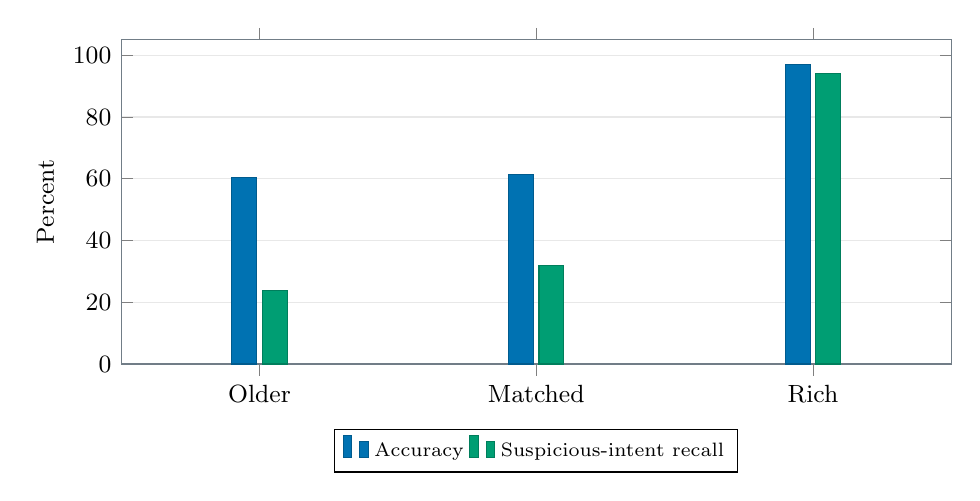
\begin{tikzpicture}
\begin{axis}[width=\columnwidth,height=5.7cm,ybar,bar width=9pt,
 ymin=0,ymax=105,ylabel={Percent},symbolic x coords={Older,Matched,Rich},
 xtick=data,ytick={0,20,40,60,80,100},
 ymajorgrids=true,grid style={gray!18},axis line style={paperInk!65},
 legend style={font=\scriptsize,at={(0.5,-0.20)},anchor=north,legend columns=2},
 tick label style={font=\small},label style={font=\small},enlarge x limits=.25]
\addplot[fill=paperBlue,draw=paperBlue!80!black] coordinates {(Older,60.51) (Matched,61.23) (Rich,97.10)};
\addplot[fill=paperTeal,draw=paperTeal!80!black] coordinates {(Older,23.70) (Matched,31.85) (Rich,94.07)};
\legend{Accuracy,Suspicious-intent recall}
\end{axis}
\end{tikzpicture}
\caption{Observed paired HTTP outcomes, not a time series or literature ranking. Rich recall remains below the 95\% release gate. The samples share a single generator and only two final peers.}
\label{httpgraph}
\end{figure}

The rich pipeline improves accuracy by 35.87 percentage points against the matched nine-feature search. It passes its predeclared large-improvement target relative to the older peer model but fails the independent release requirement. Earlier isolated-account performance of 97.94\% on 194 requests had not transferred reliably to peer-aggregated gateway observations; that failed transfer motivated causal credential context. The gain and remaining failure are both retained.

\subsection{Integrated Behavior}
A 32-case actual-service matrix yields 24 verified envelopes and eight expected HIGH-risk classical downgrade denials. MySQL joins match identifiers, versions and outcomes. All cases share one MEDIUM-scored flow; sensitivity and capabilities vary, so this is constraint coverage, not broad attack coverage.

A separate six-batch/four-client run verifies 18 envelopes and six denials with 24 matching execution/decision/event identities. Overlapping client intervals do not measure maximum throughput or internal parallelism.

The latest 44-check API/MySQL run passes. Backend packaging collects 180 tests: 175 pass, five skip, zero fail/error. Dashboard 104 tests/build and 15 rule scenarios pass. A native Prometheus probe using synthetic counter observations verifies the audit-failure rule's inactive, pending, firing and reset transitions through the administrator API. Ordinary users receive HTTP 403 and an unavailable engine returns HTTP 503 with unknown state. This is alert propagation, not real storage-fault or email-delivery proof. These checks are revision-specific functional evidence, not security percentages. Controlled Spring/H2 persistence cases do not imply actual MySQL disk-failure or ambiguous-commit evidence.

\subsubsection{Representative application outputs}
Figures~\ref{outputdecision}--\ref{outputrefusal} present complementary actual outputs from 29 October 2026: the selected policy/profile, successful PQC and hybrid verification, and an unsafe downgrade refusal. Each excerpt keeps its original displayed values while omitting navigation and unrelated panels. The associated fresh API/MySQL receipt contains 44 passing functional checks. Three additional presentation requests complete classical, hybrid and PQC envelope round trips; a fourth receives HTTP 422 because its HIGH effective risk cannot obtain an allowed quantum-resilient profile. These outputs illustrate functional behavior; the tables, measured charts and receipts provide the quantitative evaluation.

The same supplied flow receives a score of approximately 0.569 in these examples. RESTRICTED sensitivity elevates effective risk to HIGH; capability flags determine whether the allowed selection is hybrid or PQC. The classical success uses PUBLIC sensitivity with neither stronger mode supported. These fixtures demonstrate constrained selection and refusal, not recognition of four different attacks. The approximately 57\% model score is not accuracy; the excerpt's timing is one local request observation, not a benchmark estimate.

\begin{figure*}[t]
\centering
% Focus on the policy rationale; preserve the complete selected-profile/reason panel.
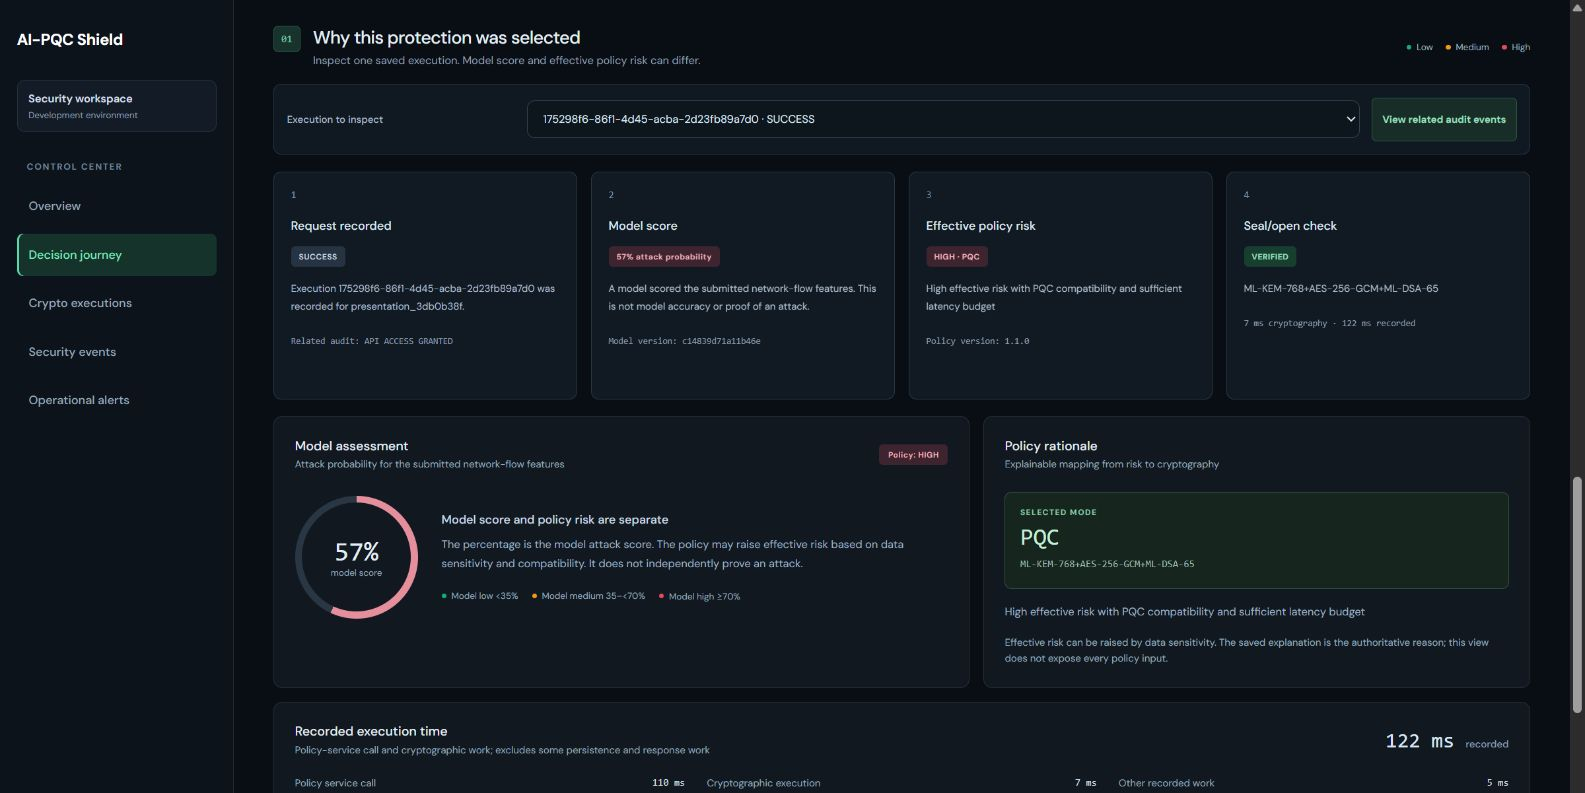
\includegraphics[width=.62\textwidth,trim=982bp 105bp 54bp 416bp,clip]{images/live-pqc-decision.jpg}
\caption{Recorded PQC policy output. The exact ML-KEM-768/AES-256-GCM/ML-DSA-65 profile and the compatibility/sensitivity rationale are retained. The panel distinguishes effective policy risk from the model score; neither is classification accuracy.}
\label{outputdecision}
\end{figure*}

\begin{figure}[t]
\centering
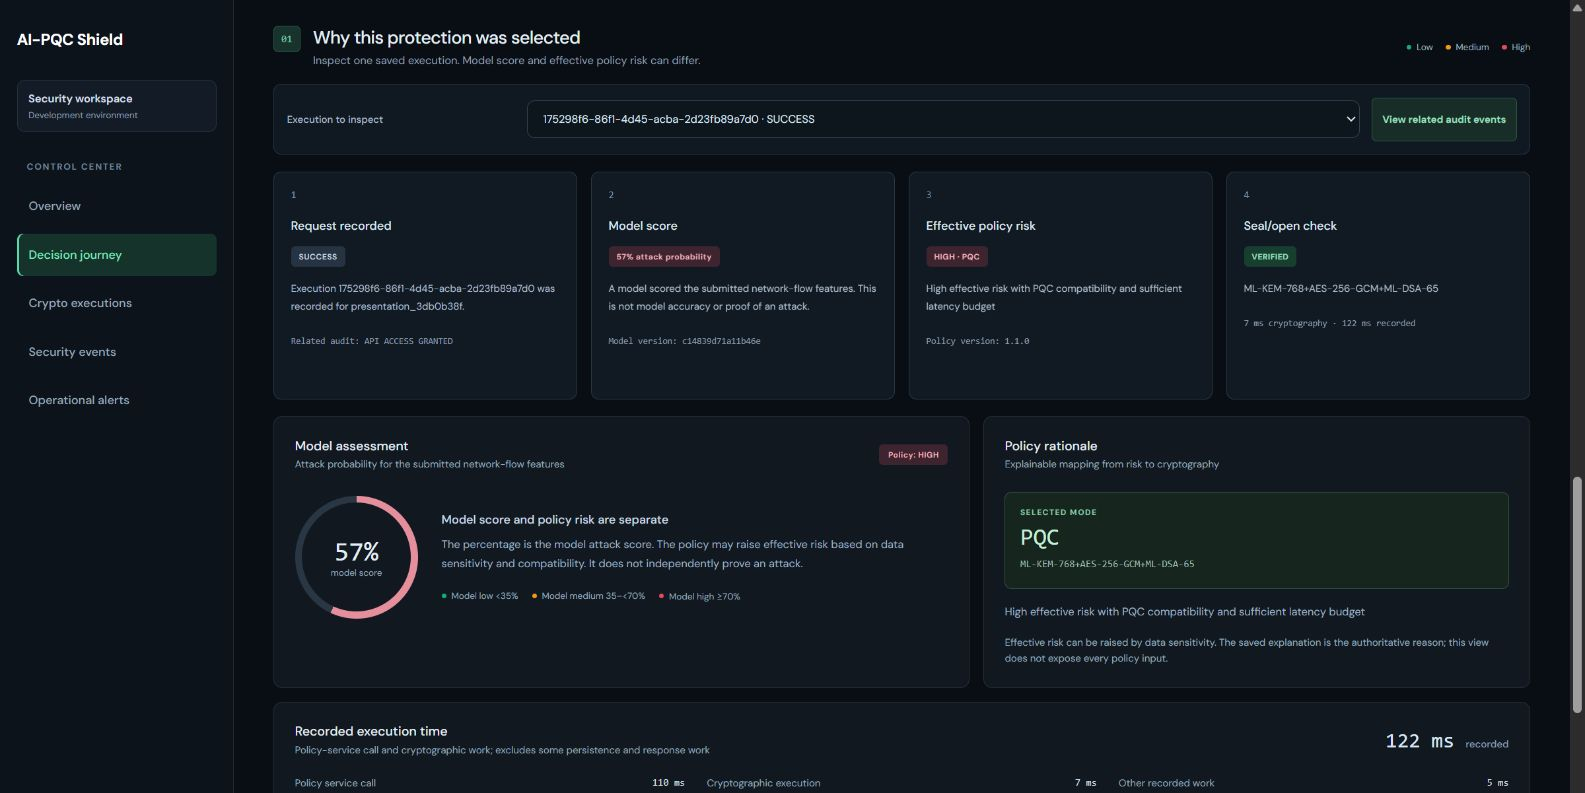
\includegraphics[width=.94\columnwidth,trim=1220bp 448bp 54bp 208bp,clip]{images/live-pqc-decision.jpg}
\caption{Actual verified PQC output. Cryptographic work took 7 ms and recorded flow time was 122 ms for this fixture only. Local round-trip verification is not deployment-wide security.}
\label{outputpqc}
\end{figure}

\begin{figure}[t]
\centering
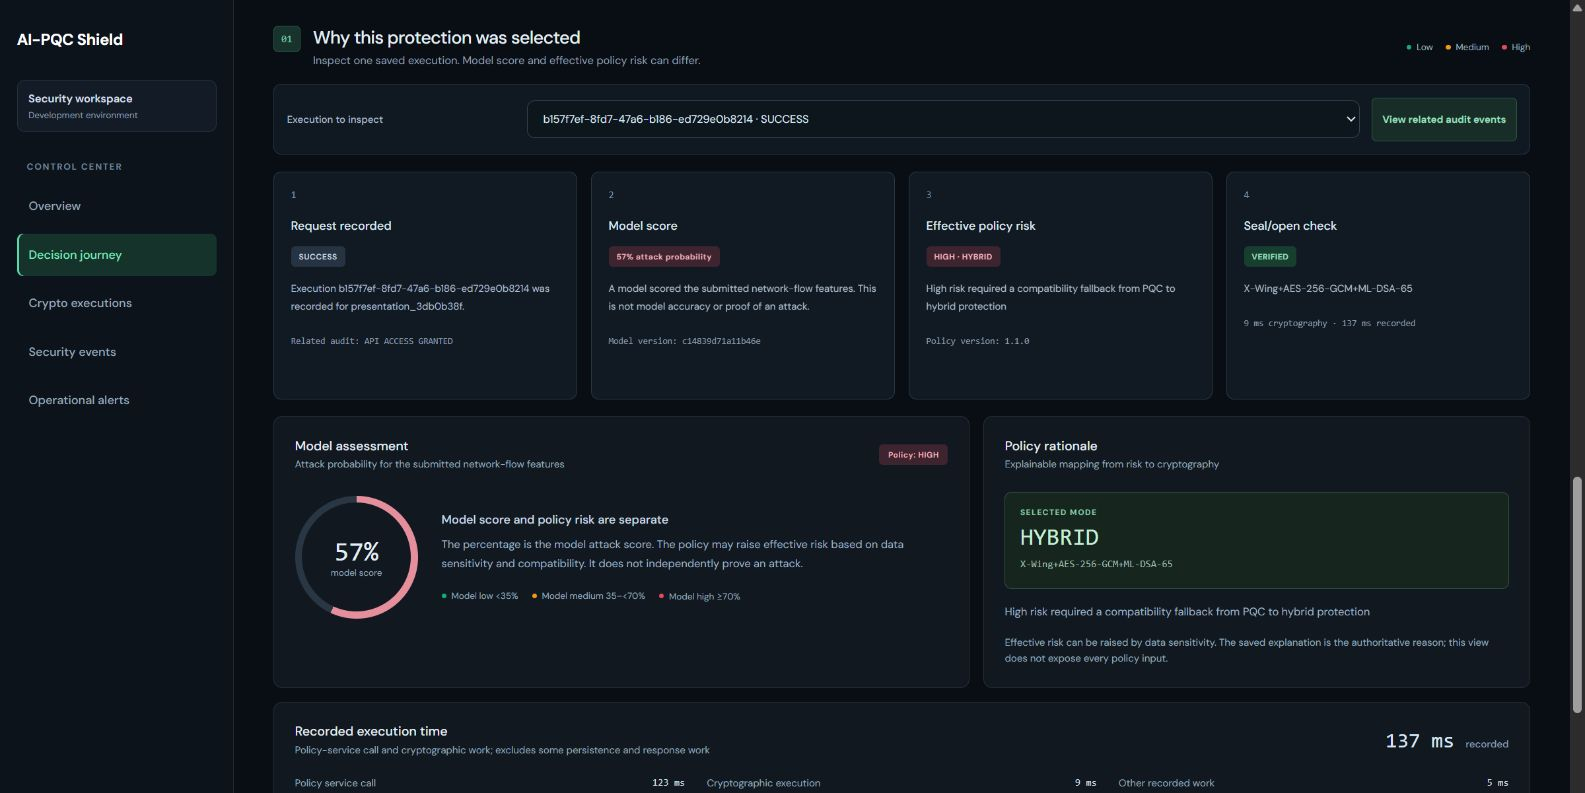
\includegraphics[width=.94\columnwidth,trim=1220bp 448bp 54bp 208bp,clip]{images/live-hybrid-decision.jpg}
\caption{Actual verified hybrid output: X-Wing/AES-256-GCM/ML-DSA-65. The same controlled run recorded 9 ms cryptographic work and 137 ms flow time; these single-request values are not benchmark estimates.}
\label{outputhybrid}
\end{figure}

\begin{figure}[t]
\centering
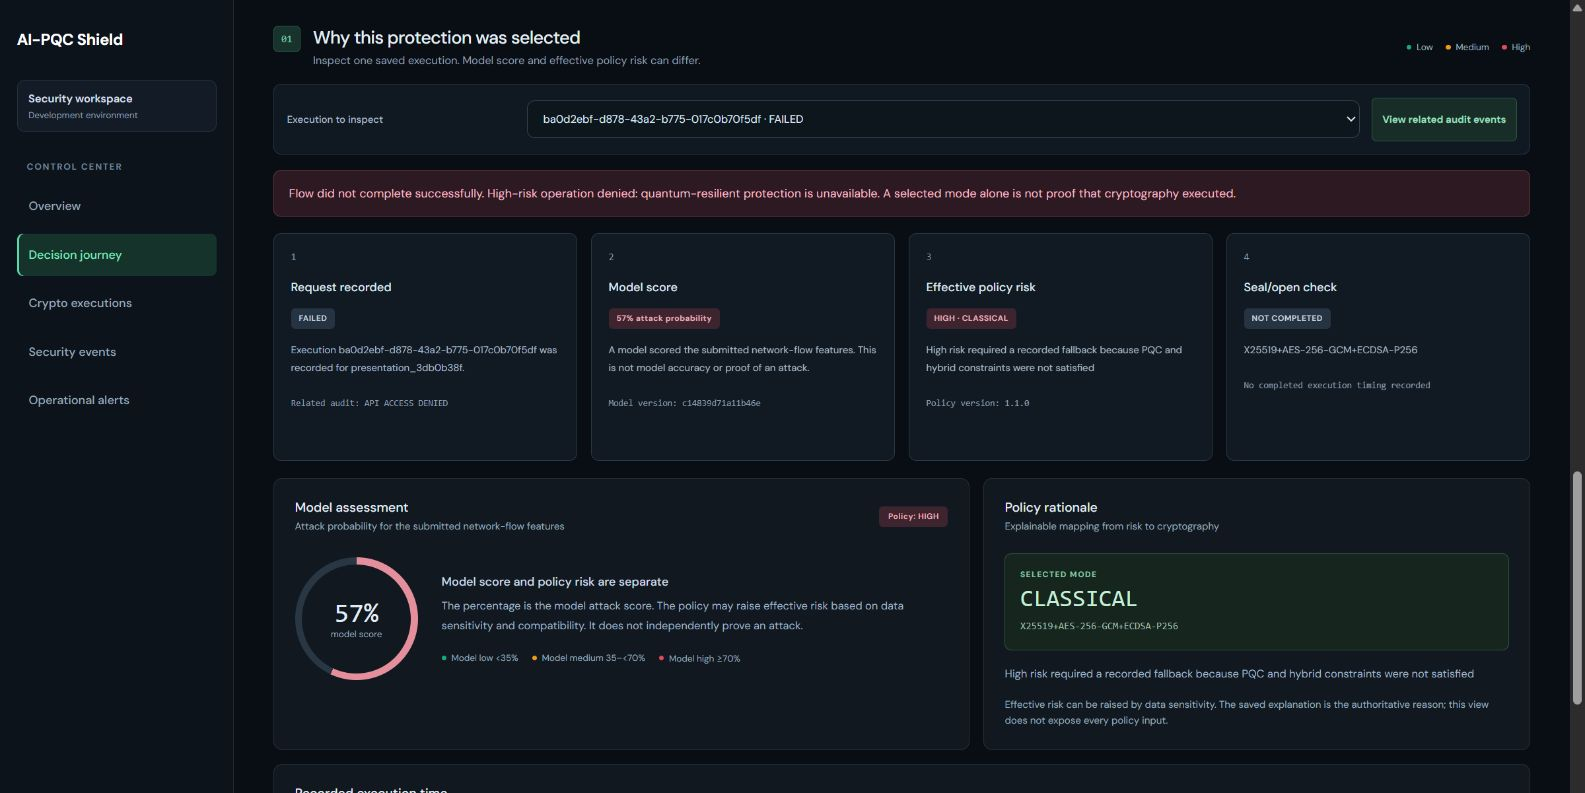
\includegraphics[width=.94\columnwidth,trim=1220bp 375bp 54bp 270bp,clip]{images/live-downgrade-refusal.jpg}
\caption{Actual refused downgrade: the HIGH-risk classical selection is NOT COMPLETED, with no completed timing. The corresponding API response is HTTP 422; a recorded selection is not successful protection.}
\label{outputrefusal}
\end{figure}

\subsubsection{What the live constraint matrix proves}
The 32 calls produce six classical, twelve hybrid and six PQC successful envelopes, alongside eight expected HTTP 422 denials. Independent read-only MySQL joins match all 32 execution, policy and event identities, versions, payload fingerprints and outcomes. This establishes consistency of the tested records rather than a dashboard-only impression. The model score is 0.5690423129295029 for every case; sensitivity and capability inputs change the effective decision. Consequently, this matrix demonstrates selected constraint branches, not that the model recognizes 32 different attacks.

The measured sequential client times range from 92.741 to 160.526 ms after readiness and ordinary verification requests. They are neither cold-start measurements nor a request-p95 estimate. Two successful zero-hint cases record crypto times of three and four milliseconds. Thus the current latency field is observably not a deadline: two of 24 successes exceed their supplied selection value. Treating its name as a performance guarantee would contradict the actual record.

The four-client experiment produces 18 verified envelopes and six expected denials, with 24 identity-consistent database joins. Overlapping client intervals establish that calls overlapped at the clients; they do not isolate internal server parallelism or find a saturation point. No capacity curve, distributed load result or adaptive-versus-static API speedup is inferred from this small run.

\subsubsection{Failure observations and operator truth}
Table~\ref{failures} records the distinct outcomes covered by the persistence tests. If initial persistence fails, policy and crypto do not run, and one sanitized failure-record attempt is made. If completion fails after actual cryptographic verification, fallback may persist FAILED with verification=true. If both completion and fallback fail, the stored STARTED record cannot establish the cryptographic outcome. The original exception is preserved with the secondary failure suppressed, and limited in-memory metrics indicate the problem.

\begin{table*}[t]
\caption{Fault evidence and interpretation. Persistence injection uses Spring/H2 transactions, not actual MySQL disk or ambiguous-commit faults.}
\label{failures}\centering\footnotesize
\begin{tabularx}{\textwidth}{|p{.22\textwidth}|p{.24\textwidth}|Y|}\hline
Tested condition & Observed durable/response contract & Supported interpretation\\\hline
Initial audit write fails & No policy/crypto execution; sanitized failure attempt; no successful response & Initiation failure prevents the protected operation under the controlled path\\\hline
Crypto passes; completion enqueue fails once & Completion rolls back; fallback FAILED/verified=true; no returned envelope & A verified envelope does not imply a successful completed business flow\\\hline
Completion and fallback both fail & Earlier STARTED remains; original exception retained; failure counter increments & Durable completion is unknown; metrics do not repair the missing record\\\hline
Synthetic audit metric becomes positive & Actual Prometheus pending/firing state reaches admin API & Rule propagation works for the injected metric, not proof of a real DB incident\\\hline
Monitoring engine unavailable & API returns 503 / unknown; ordinary user returns 403 & Unavailable state is not presented as healthy or exposed to ordinary users\\\hline
\end{tabularx}
\end{table*}

In the live monitoring probe, the synthetic counter is observed inactive at approximately 5.72 s, pending at 11.96 s, firing at 27.63 s and inactive at 29.73 s after a simulated counter reset. The restricted API exposes corresponding transitions. These are elapsed observations from one probe, not an alert-delivery SLA. Resetting a synthetic counter is not incident recovery; a real counter's process lifecycle and unsampled failures require separate handling. Local test sinks do not establish email arrival at an external recipient.

\subsection{Matched Local Cryptographic Workload}
Table~\ref{timing} and Fig.~\ref{cryptograph} report the same complete-envelope operation boundary for all three profiles. The machine is an Intel i7-13650HX laptop with 16 GB installed memory, JVM 21.0.12.1 and Bouncy Castle 1.86. The run completes in 236.78 s. Power state, thermals, CPU affinity and background activity are not controlled, and profile order is sequential. This is a reproducible development checkpoint rather than an isolated performance laboratory.

\begin{table}[t]
\caption{Fresh-key 4 KiB envelope workload; JMH average time}
\label{timing}\centering\footnotesize
\begin{tabular}{|l|r|r|r|}\hline
Profile & Mean ms/op & 99.9\% JMH interval & B/op\\\hline
Classical &8.057&7.315--8.799&169,486\\\hline
Hybrid &6.685&6.525--6.845&710,814\\\hline
PQC &5.309&5.211--5.406&677,170\\\hline
\end{tabular}
\end{table}

\begin{figure}[t]
\centering
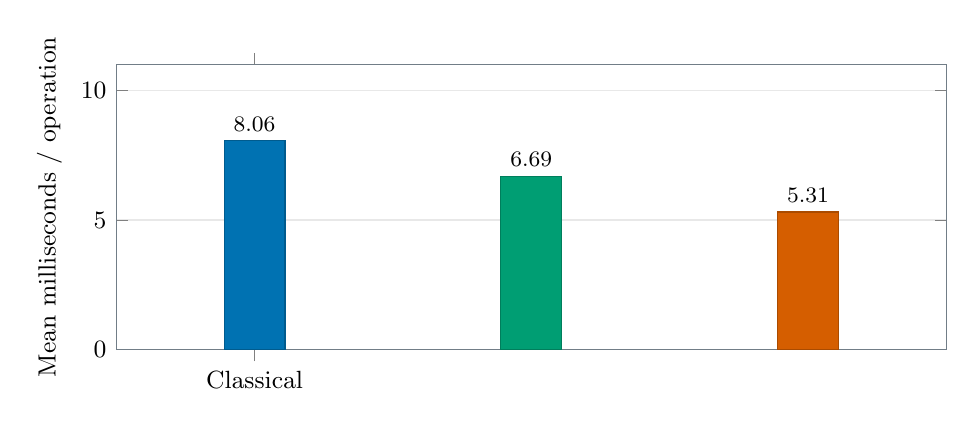
\begin{tikzpicture}
\begin{axis}[width=\columnwidth,height=5.2cm,ybar,bar width=22pt,
 ymin=0,ymax=11,ylabel={Mean milliseconds / operation},
 symbolic x coords={Classical,Hybrid,PQC},xtick=data,
 ymajorgrids=true,grid style={gray!18},axis line style={paperInk!65},
 tick label style={font=\small},label style={font=\small},enlarge x limits=.25,
 nodes near coords,nodes near coords style={font=\footnotesize}]
\addplot[bar shift=0pt,fill=paperBlue,draw=paperBlue!80!black] coordinates {(Classical,8.057)};
\addplot[bar shift=0pt,fill=paperTeal,draw=paperTeal!80!black] coordinates {(Hybrid,6.685)};
\addplot[bar shift=0pt,fill=paperOrange,draw=paperOrange!80!black] coordinates {(PQC,5.309)};
\end{axis}
\end{tikzpicture}
\caption{Measured fresh-key envelope path, including setup, encryption, signing, opening and verification. Table~\ref{timing} gives JMH intervals. These are not API latency, request tail latency or comparable security-strength scores.}
\label{cryptograph}
\end{figure}

Classical fork means range from 6.727 to 10.070 ms, hybrid from 6.528 to 7.000 ms and PQC from 5.168 to 5.442 ms. The larger classical variation warns against interpreting a single mean as an invariant ordering. JMH's intervals describe the recorded benchmark score under its estimator; they do not cover arbitrary hosts, future JVMs or deployed request distributions. Fifty iteration means are not fifty independent request-latency observations, so no request p95 or p99 is computed from them.

The PQC path is faster in this measured fresh-key workload while allocating more bytes than classical. That statement is intentionally local. Key lifecycle, implementations and profile primitives differ; an equal operation boundary does not equalize security strength. No profiling result attributes the difference to a specific primitive. No conclusion that PQC is generally faster, or that adaptation accelerates a business workload, follows from these measurements.

Table~\ref{sizes} reports separate raw component samples. The classical encapsulation length is this implementation's encoded representation, not a claim that an X25519 raw public key has that length. ECDSA signatures vary across the 16 samples. All totals exclude metadata, keys, JSON/base64, HTTP/TLS and framing. They therefore describe component storage in the measured envelope, not bytes transmitted over a production link.

\begin{table}[t]
\caption{Observed component sizes for a 4,096-byte payload, bytes}
\label{sizes}\centering\footnotesize
\begin{tabular}{|l|r|r|r|r|}\hline
Profile & Encaps. & Nonce & Ciphertext & Signature\\\hline
Classical &44&12&4,112&70--72\\\hline
Hybrid &1,120&12&4,112&3,309\\\hline
PQC &1,088&12&4,112&3,309\\\hline
\multicolumn{5}{|l|}{Raw totals: 4,238--4,240; 8,553; 8,521, respectively.}\\\hline
\end{tabular}
\end{table}

\subsection{Answers to the Research Questions}
RQ1 is supported within the frozen scenarios: implemented profiles execute, unsafe HIGH/classical fallbacks are refused and corresponding records agree. It is not answered for arbitrary risk flows or untrusted telemetry. RQ2 shows that promising validation or isolated-account accuracy does not reliably transfer, while richer causal HTTP context yields a substantial paired laboratory gain without meeting release recall. The syscall ablations provide no eligible replacement. RQ3 establishes that cryptographic verification, durable completion and observable alert state must remain separate; some combined failures leave an ambiguous durable state. RQ4 is answered only for the measured fresh-key envelope boundary, with explicit timing and size limitations. No question is converted into a universal security percentage.

\section{Discussion}
The results expose two related risks: overstating generalization from a convenient split, and overstating system protection from a successful component. Both require explicit evidence boundaries.

\subsection{Detection Is Not an Encryption Policy by Itself}
An attack score cannot determine every protection requirement. A low-scored medical or financial record may need a long confidentiality lifetime, whereas repeated invalid logins mainly require authentication controls and carefully bounded throttling. Raising the cryptographic cost of each hostile request can consume additional resources without rejecting the attack. Our tested policy demonstrates profile selection and downgrade rejection; it does not prove an optimal response to adversarial demand.

A production policy should establish a resource-owned minimum cryptographic floor independently of a caller's score. Model observations could then influence additional controls without weakening the required confidentiality. The prototype's public/internal branches are useful for demonstrating agility but should not be interpreted as a complete enterprise migration strategy. Migration planning in~\cite{readiness} and algorithm abstraction in~\cite{enterprise} concern dependencies and data lifetime beyond the current request. This is a reason to keep migration state, detector state and access state separate.

The same principle applies to availability. A bounded local authentication burst returned ten HTTP 401 responses and two HTTP 429 responses in a twelve-request case; spoofed forwarding headers did not bypass the tested peer-based limit. That is a useful local control, not distributed DDoS protection or evidence against large botnets. Multiple peers, proxy topology, legitimate shared clients and service saturation need different experiments. PQC cannot repair an exhausted request queue, and a classifier should not be credited for a deterministic authentication rejection.

\subsection{Why More Training Was Not the Next Experiment}
The microservice ablations already test several ways to expose additional information. Generic errors slightly reduce selected-control alarms while losing an exposure hit. Rich features and short causal history do not meet recall gates. Exact cross-label vectors and the concentrated difficult CVE indicate that the next question concerns what was observed and what the interval annotation means. Another parameter sweep on the same windows could improve a development score without establishing that the detector sees the intended attack.

Accordingly, this paper does not add an ``extreme'' training run merely to pursue a percentage target. A justified next study would first validate target coverage, timing alignment and behavior-specific annotations, then declare a representation and candidate budget before opening independent scenarios. A detector using a longer context or different sensor might be valuable, but it would answer a new measurement question. Correcting genuine preparation errors is legitimate; deleting difficult cases or relabeling misses to improve recall is not.

The HTTP result illustrates a more productive form of iteration. A causal context hypothesis addresses a concrete representation weakness, and its gain is measured on identical final requests against a matched search. Even then, the result remains below the required recall. This separation between an informative improvement and a release decision is central to reliable experimentation. The paper records both, avoiding the assumption that every iteration must produce a deployable model.

\subsection{Practical MLOps and Versioned Evidence}
The project's local-first workflow includes training scripts, experiment records, model hashes, frozen recipes and explicit candidate retention. These are MLOps mechanisms insofar as they support reproducibility and controlled promotion, consistent with separating application, policy and observability concerns in the microservice lifecycle~\cite{devsecops}. They are not evidence of an autonomous self-healing learning system. A rejected candidate remains experimental; changing the serving model or enabling automatic blocking requires a separate accepted release decision.

Model, schema and policy versions must travel with a decision because each can change its interpretation. A score computed using an incompatible feature order is not repaired by an accurate model name. A valid prediction processed by an unrecorded policy revision is difficult to reproduce. Similarly, retraining on new data without preserving the old artifact would undermine rollback and historical audit. The versioned execution record therefore serves both software operations and research interpretation.

NIST's distinction among policy, observability and application code~\cite{devsecops} explains why the evidence pack spans more than ML outputs. Test-rule changes, API authorization, transaction behavior and dashboard interpretation can alter what an operator believes without changing a single model parameter. The controlled post-crypto failure exposed such a problem: a UI contract initially rejected a valid FAILED/verified=true state. Correcting the interpretation was a security-relevant improvement even though it added no classification accuracy.

\subsection{Threats to Validity}
\subsubsection{Construct validity}
Network attack labels, suspicious HTTP intent and syscall exposure are not interchangeable ground truth. An exposure hit does not prove exploit prevention, and a correct denial does not prove a model recognized an attack. A local seal/open verifies computation under the generated keys, not identity assurance between independent endpoints. These distinctions are retained in table captions and result denominators to reduce construct inflation.

\subsubsection{Internal validity}
Training-only transformation fitting and frozen candidate recipes reduce some leakage risks, but they do not eliminate all dependence. CIC ranges may share capture context. SocialNetwork windows are correlated and repeatedly inspected during development. The rich and base HTTP searches choose different estimators, so their gain cannot be attributed only to a feature addition. Benchmark profile ordering and background host activity can influence performance. No randomized end-to-end comparison isolates adaptation as the cause of lower latency or improved security.

\subsubsection{External validity}
The public datasets represent their own environments, not arbitrary microservice applications. The local request generator, two final peers and synthetic payload do not represent an internet deployment. Service discovery, proxy behavior, key management, storage failure and adversarial traffic can differ substantially on a hosted platform. The results support a local prototype with known limits, not a commercial service-level guarantee, broad compatibility certification or a quantified probability of surviving unknown attacks.

\subsubsection{Statistical conclusion validity}
Accuracy depends on prevalence, and macro-F1 remains sensitive to finite support. The selected-control ratio in the syscall study is artificial. Small scenario counts can make a percentage appear more stable than the underlying evidence. JMH intervals describe its recorded operation estimator, not request-tail uncertainty. We therefore present confusion counts, support sizes, fork variation and gate outcomes rather than combining all tests into a single reassuring percentage.

\subsection{A Bounded Next Evaluation}
The next deployment-oriented experiment should compare fixed classical, fixed hybrid, fixed PQC and adaptive execution on the same declared workload, while enforcing identical safety floors. It should separately measure request-level latency, tail behavior, resource consumption, refusal rate, policy cost, inference cost, database cost and outbox delay. Randomized or counterbalanced execution order and repeated runs would help distinguish profile effects from host drift. This is proposed work, not a result of the present study.

For detection, independent microservice traffic should include legitimate bursts, software updates, shared peers, credential rotation and hard negative examples. Group definitions and labels must be fixed before scoring. Trusted collection should attach observations to actual requests rather than accepting arbitrary caller features. An initial shadow phase can measure false alarms without giving an unaccepted candidate authority to block users. External email, persistent incidents and alert recovery also require their own end-to-end acceptance checks.

The resulting evaluation should preserve rejected candidates as well as successful cases. A matched improvement over a reproducible baseline would be useful, but absence of such a gain does not justify hiding failed candidates. The present evidence supports an auditable integration study with negative generalization findings. Future extensions can reuse its separation of classification, constrained selection, cryptographic verification and durable outcome rather than inheriting a single ambiguous success metric.

\section{Conclusion}
The central finding is that a security framework needs several kinds of evidence, not one headline accuracy. The retained network RF provides high attack recall with a high false-positive rate. The bounded IoT candidates and grouped syscall studies do not meet their gates. Rich causal HTTP context yields a substantial paired improvement but still misses final recall. Actual-service tests support specific profile and record contracts, while controlled failure tests show why cryptographic verification cannot stand in for durable completion. Matched envelope timings characterize one local workload without establishing a production advantage.

Future work should prioritize authoritative telemetry, behavior-aligned labels, authenticated key delivery and independently evaluated failure recovery. Stronger claims require those missing boundaries to be tested rather than inferred from algorithm names or successful screenshots. Within its stated scope, the prototype offers an executable basis for investigating adaptive, crypto-agile microservice protection and for preserving the limitations needed to reproduce its findings.

\section*{Acknowledgment}
The authors acknowledge the creators of the public datasets and open-source tools used in this study. Dataset and standards sources are cited where their methods or artifacts are used.

\appendices
\section{Reproduction and Artifact Map}
The manuscript is based on versioned project reports and retained local receipts rather than screenshots. Raw datasets, research PDFs, model binaries, credentials and extracted full text are not committed with the source. Table~\ref{artifactmap} maps result families to the tracked study documents. Their receipts identify the exact local inputs, outputs and code revisions. A fresh run should use a new output directory so that an earlier failed or interrupted attempt is not overwritten.

\begin{table*}[t]
\caption{Project evidence map. Paths are relative to \texttt{docs/research/}; these are project records, not external literature.}
\label{artifactmap}\centering\footnotesize
\begin{tabularx}{\textwidth}{|p{.25\textwidth}|Y|}\hline
Claim family & Tracked study record\\\hline
Official network baseline & \path{phase-3-baseline-results.md}\\\hline
Bounded IoT final evaluation & \path{ciciot2023-final-results.md}; \path{evidence/ciciot2023-frozen-final-v1.json}\\\hline
Grouped syscall expansion & \path{socialnetwork-development-expansion-v1.md}\\\hline
Causal history / exploratory guard & \path{socialnetwork-temporal-study-v1.md}\\\hline
Generic errors / feature ambiguity & \path{socialnetwork-errors-results-v1.md}\\\hline
Paired HTTP comparison & \path{rich-context-http-v1.md}; \path{evidence/rich-context-http-v1.json}\\\hline
Actual-service constraint matrix & \path{adaptive-matrix-results-v1.md}\\\hline
Overlapping client calls & \path{concurrent-adaptive-results-v1.md}\\\hline
Persistence failure semantics & \path{initial-audit-failure-results-v1.md}; \path{post-crypto-audit-results-v1.md}\\\hline
Alert propagation & \path{adaptive-audit-alert-live-results-v1.md}\\\hline
Complete-envelope benchmark & \path{matched-envelope-results-v1.md}\\\hline
\end{tabularx}
\end{table*}

The promoted model is identified by SHA-256 beginning \texttt{c14839d71a11b46e}; the full digest is retained in the evidence. This is an artifact identity, not a guarantee of suitability. The network baseline environment records Python 3.14.6, pandas 3.0.6, scikit-learn 1.9.1, joblib 1.6.0 and MLflow 3.16.1. Later bounded studies retain their own dependency versions, including XGBoost 3.4.1. They should not be silently rerun under different packages and assumed numerically identical.

Reproduction proceeds in stages. First, obtain the cited data under its applicable terms and verify the publisher/local checksums. Second, reproduce schema checks and preparation with the recorded partition boundaries. Third, inspect the frozen recipe before fitting and keep transformation state inside the training pipeline. Fourth, reproduce development checks without opening an exposed final test for new selection. A genuinely new confirmatory evaluation needs a new independent partition and a declared recipe, not a repeat of model selection on old results.

For system checks, start service dependencies with local secrets supplied outside tracked source, wait for explicit readiness, and run the frozen synthetic request cases. Save client receipts before making independent read-only database joins. Preserve identifiers, versions and outcomes; do not save bearer credentials or private keys as evidence. Stop only processes created for the test. Interrupted attempts without completed receipts remain unverified rather than being counted as passes or silently discarded.

For the JMH study, retain the shaded executable hash, JVM/provider versions, fork protocol, raw JSON, allocation units and separate size samples. Aggregation verifies the number of profiles and iteration means and recomputes component totals. A plot should use those recorded values; an unmeasured throughput curve, learning curve or p99 chart is not a substitute. A rerun under controlled hardware would be a new result with its own provenance, not a cosmetic replacement of this one.

\section{Interpretation and Reporting Rules}
Reporting preserves three boundaries: the evaluated unit, the data split and the component outcome. Flow recall, window exposure hits and functional passes have different denominators. Validation gains are not official-test gains; reused development folds are not independent confirmation. Selected mode, verified envelope, completed request and delivered event remain distinct states.

Dashboard language follows these boundaries. An absent alert may reflect healthy, missing, stale or unavailable observations. A selected mode does not establish deployment security, and a model score is not compromise probability. Unestablished outcomes are reported as unknown rather than inferred successful.

Data availability follows publisher licenses. Local observations are controlled synthetic requests and derived features, not customer traffic. Reproduction packets preserve scenario definitions, dependency versions and hashes while excluding credentials and private material. Changed preparation or observation boundaries must be reported explicitly.

\balance
\begin{thebibliography}{00}
\bibitem{mesh} R. Chandramouli and Z. Butcher, \emph{Building Secure Microservices-based Applications Using Service-Mesh Architecture}, NIST SP 800-204A, 2020, doi:10.6028/NIST.SP.800-204A.
\bibitem{kem} NIST, \emph{Module-Lattice-Based Key-Encapsulation Mechanism Standard}, FIPS 203, 2024, doi:10.6028/NIST.FIPS.203.
\bibitem{dsa} NIST, \emph{Module-Lattice-Based Digital Signature Standard}, FIPS 204, 2024, doi:10.6028/NIST.FIPS.204.
\bibitem{gateway} M. Matias, E. Ferreira, N. Mateus-Coelho, O. Ribeiro, and L. Ferreira, \emph{Evaluating Effectiveness and Security in Microservices Architecture}, Procedia Computer Science, vol. 237, pp. 626--636, 2024, doi:10.1016/j.procs.2024.05.148.
\bibitem{readiness} A. Gupta and S. Mittal, \emph{Post-quantum readiness and cryptographic transition planning for enterprise cloud}, Cybersecurity, vol. 9, art. 147, 2026, doi:10.1186/s42400-026-00579-2.
\bibitem{enterprise} M. V. Inakollu, \emph{Quantum-Resilient Architectures for Enterprise and Cloud Information Systems, Implications of Quantum Computing for Enterprise Cybersecurity and Data Integrity}, Acta Sci., vol. 26, no. 3, 2025, doi:10.22178/acta.26.3.44. Retained repository copy: \url{https://digitalcommons.usf.edu/esb_facpub/161}.
\bibitem{unsw} N. Moustafa and J. Slay, \emph{UNSW-NB15: a comprehensive data set for network intrusion detection systems (UNSW-NB15 network data set)}, Proc. MilCIS, 2015. \url{https://research.unsw.edu.au/projects/unsw-nb15-dataset}.
\bibitem{ciciot} E. C. P. Neto et al., \emph{CICIoT2023: A Real-Time Dataset and Benchmark for Large-Scale Attacks in IoT Environment}, Sensors, vol. 23, no. 13, art. 5941, 2023, doi:10.3390/s23135941.
\bibitem{flora} J. Flora and N. Antunes, \emph{Evaluating intrusion detection for microservice applications: Benchmark, dataset, and case studies}, Journal of Systems and Software, vol. 216, art. 112142, 2024, doi:10.1016/j.jss.2024.112142.
\bibitem{dataset} J. Flora and N. Antunes, \emph{Microservice Intrusion Detection Dataset}, Zenodo, ver. 0.0.1, 2024, doi:10.5281/zenodo.10655126.
\bibitem{adaptive} F. G. Stasac, C. A. Gy{\H{o}}r{\"o}di, and R. S. Gy{\H{o}}r{\"o}di, \emph{Adaptive Encryption Framework for Web Applications: A Risk-Based Approach to Dynamic Algorithm Selection}, Applied Sciences, vol. 16, no. 17, art. 8889, 2026, doi:10.3390/app16178889.
\bibitem{sage} H. D. Binh, Y.-h. Choi, J. Jeong, Y.-J. Lee, and D. Shin, \emph{A Study on a Network Intrusion Detection System Based on the Fusion of SAGEConv-GNN and a Transformer Encoder}, Electronics, vol. 15, no. 8, art. 1737, 2026, doi:10.3390/electronics15081737.
\bibitem{session} A. Olushola and S. P. Meenakshi, \emph{Design and implementation of an authenticated post-quantum session protocol using ML-KEM (Kyber), ML-DSA (Dilithium), and AES-256-GCM}, Frontiers in Physics, vol. 13, art. 1723966, 2026, doi:10.3389/fphy.2025.1723966.
\bibitem{devsecops} R. Chandramouli, \emph{Implementation of DevSecOps for a Microservices-based Application with Service Mesh}, NIST SP 800-204C, Mar. 2022, doi:10.6028/NIST.SP.800-204C.
\bibitem{feature} Z. Asghari Varzaneh and S. Hosseini, \emph{An improved equilibrium optimization algorithm for feature selection problem in network intrusion detection}, Scientific Reports, vol. 14, art. 18696, 2024, doi:10.1038/s41598-024-67488-7.
\bibitem{xai} K. P. Sharma et al., \emph{Interpretable intrusion detection for IoT environments using a self-attention-based explainable AI framework}, Scientific Reports, vol. 15, art. 39937, 2025, doi:10.1038/s41598-025-23750-0.
\end{thebibliography}
\end{document}
